\documentclass[border=4pt]{standalone}\usepackage[utf8]{inputenc}\usepackage[T1]{fontenc}\usepackage{mathptmx}
\usepackage{tikz}
\usetikzlibrary{arrows.meta,positioning,calc,fit,backgrounds}
\tikzset{>={Stealth[length=2.2mm]}, font=\small,
 blk/.style={draw, line width=0.8pt, fill=white, align=center, inner sep=3pt, text width=#1, minimum height=1.1cm},
 blk/.default=3.0cm,
 iut/.style={fill=black!14},
 ext/.style={draw, dashed, line width=0.5pt, align=center, inner sep=3pt, text width=#1, minimum height=1.0cm, fill=white},
 ext/.default=2.6cm,
 grp/.style={draw=black!55, dashed, line width=0.5pt, fill=black!4, inner sep=7pt},
 glab/.style={font=\small\itshape, text=black!75, anchor=north west, inner sep=2pt},
 lab/.style={font=\footnotesize, inner sep=1.5pt, fill=white},
 pw/.style={line width=2.2pt, -{Stealth[length=2.6mm]}},
 dg/.style={line width=0.6pt},
 an/.style={line width=0.8pt, dashed},
 rf/.style={double, double distance=1.2pt, line width=0.4pt},
 cd/.style={line width=0.6pt, dotted}}

\begin{document}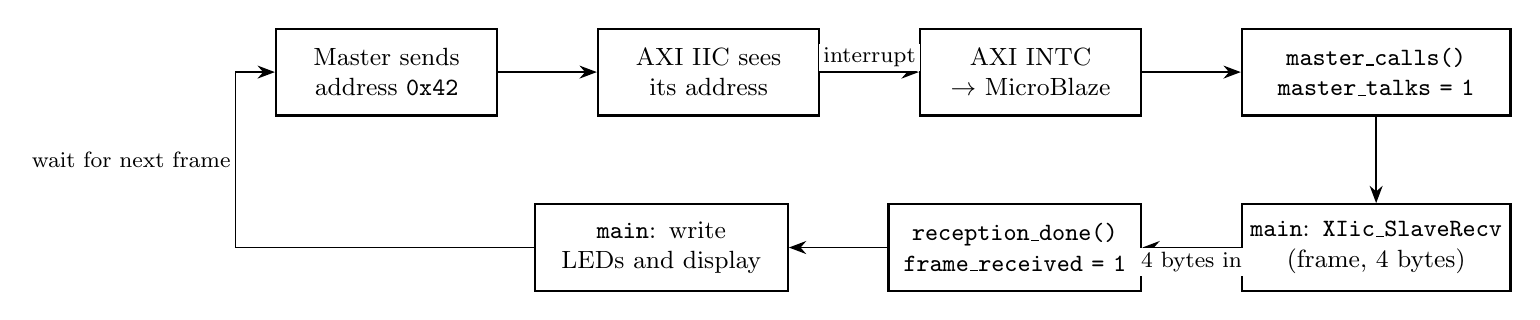
\begin{tikzpicture}[node distance=1.25cm]
\node[blk=2.6cm] (m) {Master sends\\address \texttt{0x42}};
\node[blk=2.6cm, right=of m] (iic) {AXI IIC sees\\its address};
\node[blk=2.6cm, right=of iic] (intc) {AXI INTC\\$\rightarrow$ MicroBlaze};
\node[blk=3.2cm, right=of intc] (h1) {\texttt{master\_calls()}\\\texttt{master\_talks = 1}};
\node[blk=3.2cm, below=1.1cm of h1] (rx) {\texttt{main}: \texttt{XIic\_SlaveRecv}\\(frame, 4 bytes)};
\node[blk=3.0cm, left=of rx] (h2) {\texttt{reception\_done()}\\\texttt{frame\_received = 1}};
\node[blk=3.0cm, left=of h2] (out) {\texttt{main}: write\\LEDs and display};
\draw[dg,->] (m) -- (iic); \draw[dg,->] (iic) -- node[lab,above]{interrupt} (intc);
\draw[dg,->] (intc) -- (h1); \draw[dg,->] (h1) -- (rx);
\draw[dg,->] (rx) -- node[lab,below]{4 bytes in} (h2); \draw[dg,->] (h2) -- (out);
\coordinate (lx) at ($(m.west)+(-0.5,0)$);
\draw[dg,->] (out.west) -- (out.west -| lx) -- node[lab,left]{wait for next frame} (lx) -- (m.west);
\end{tikzpicture}\end{document}
